{
\abnormalparskip{0pt}
\chapter{Discussion}
\label{cha:discussion}
}

\TODO[inline]{Write discussion}

concurrent/parallel gauss-elimination or run of the algorithm. We would have to
sync only the upperbound. would have to make a copy() function due to golangs
structs. this could be memory intensive?

Other ways of sorting the terminals?

Lower bounds? these however seem to all be very complex.

Lad analytisk metode propagerer sine changes ud fra nyt steiner punkt, og
evt. tilbage igen

Placer punkter m. analytisk metode i stedet for med perturberet centroid.

Kører iteration kun på den del der er blevet ændret, dvs. kun de FSTs der er
affekteret af det fulde FST.

\subsection{Concurrency}
\label{sec:concurrency}

\begin{figure}[htbp]
  \centering
  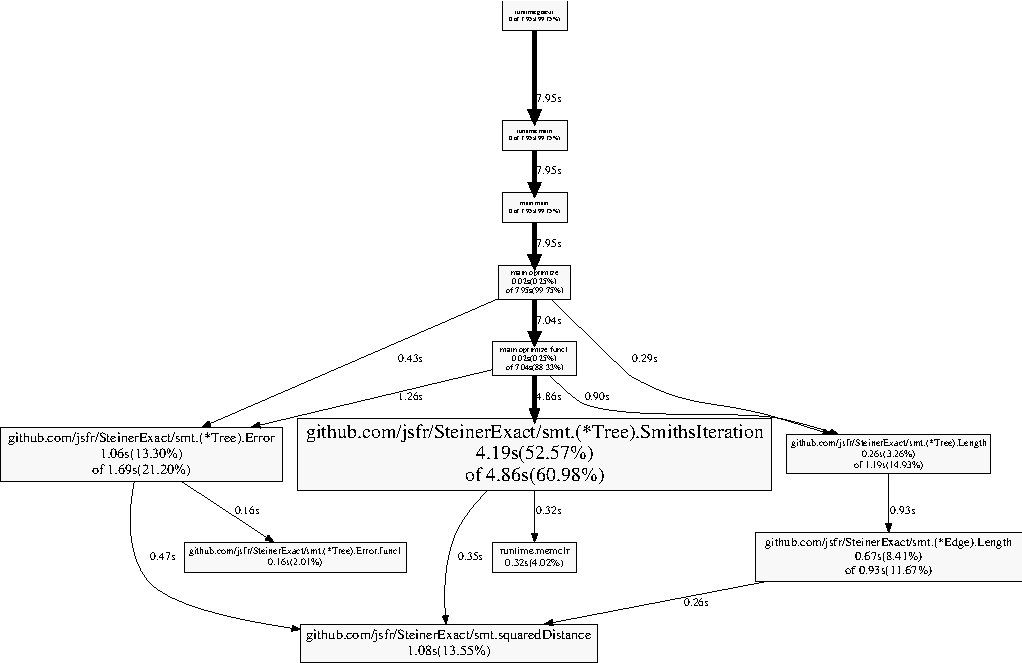
\includegraphics[width=\textwidth]{gfx/pprof001}
  \caption[CPU-time profile of a single execution]{Here be dragons\label{fig:pprof}}
\end{figure}

%%% Local Variables:
%%% mode: latex
%%% TeX-master: "../../main"
%%% End:
